\subsection{bestLDS infers correct parameters on simulated datasets}
\label{sec:bestlds:results:4.1}

We begin by illustrating the effectiveness of the moment conversion for a very high-dimensional system (observation dimension $q = 30$, latent dimension $p = 15$, Hankel parameter $k =20$, and input dimension $m=3$). We sampled from a probit-Bernoulli LDS model and display the sample covariance of the observations, $\mathrm{cov}[y_t, y_{t+1}]$, the transformed covariance of the latents obtained by moment conversion, $\mathrm{cov}[z_{t}, z_{t+1}]$ as well as the true latent covariance matrix (Figure ~\ref{fig:bestlds:2}a). Observe that the output covariance does not match the latent covariance, while the converted moments do.

\begin{figure*}[t!]
\centering
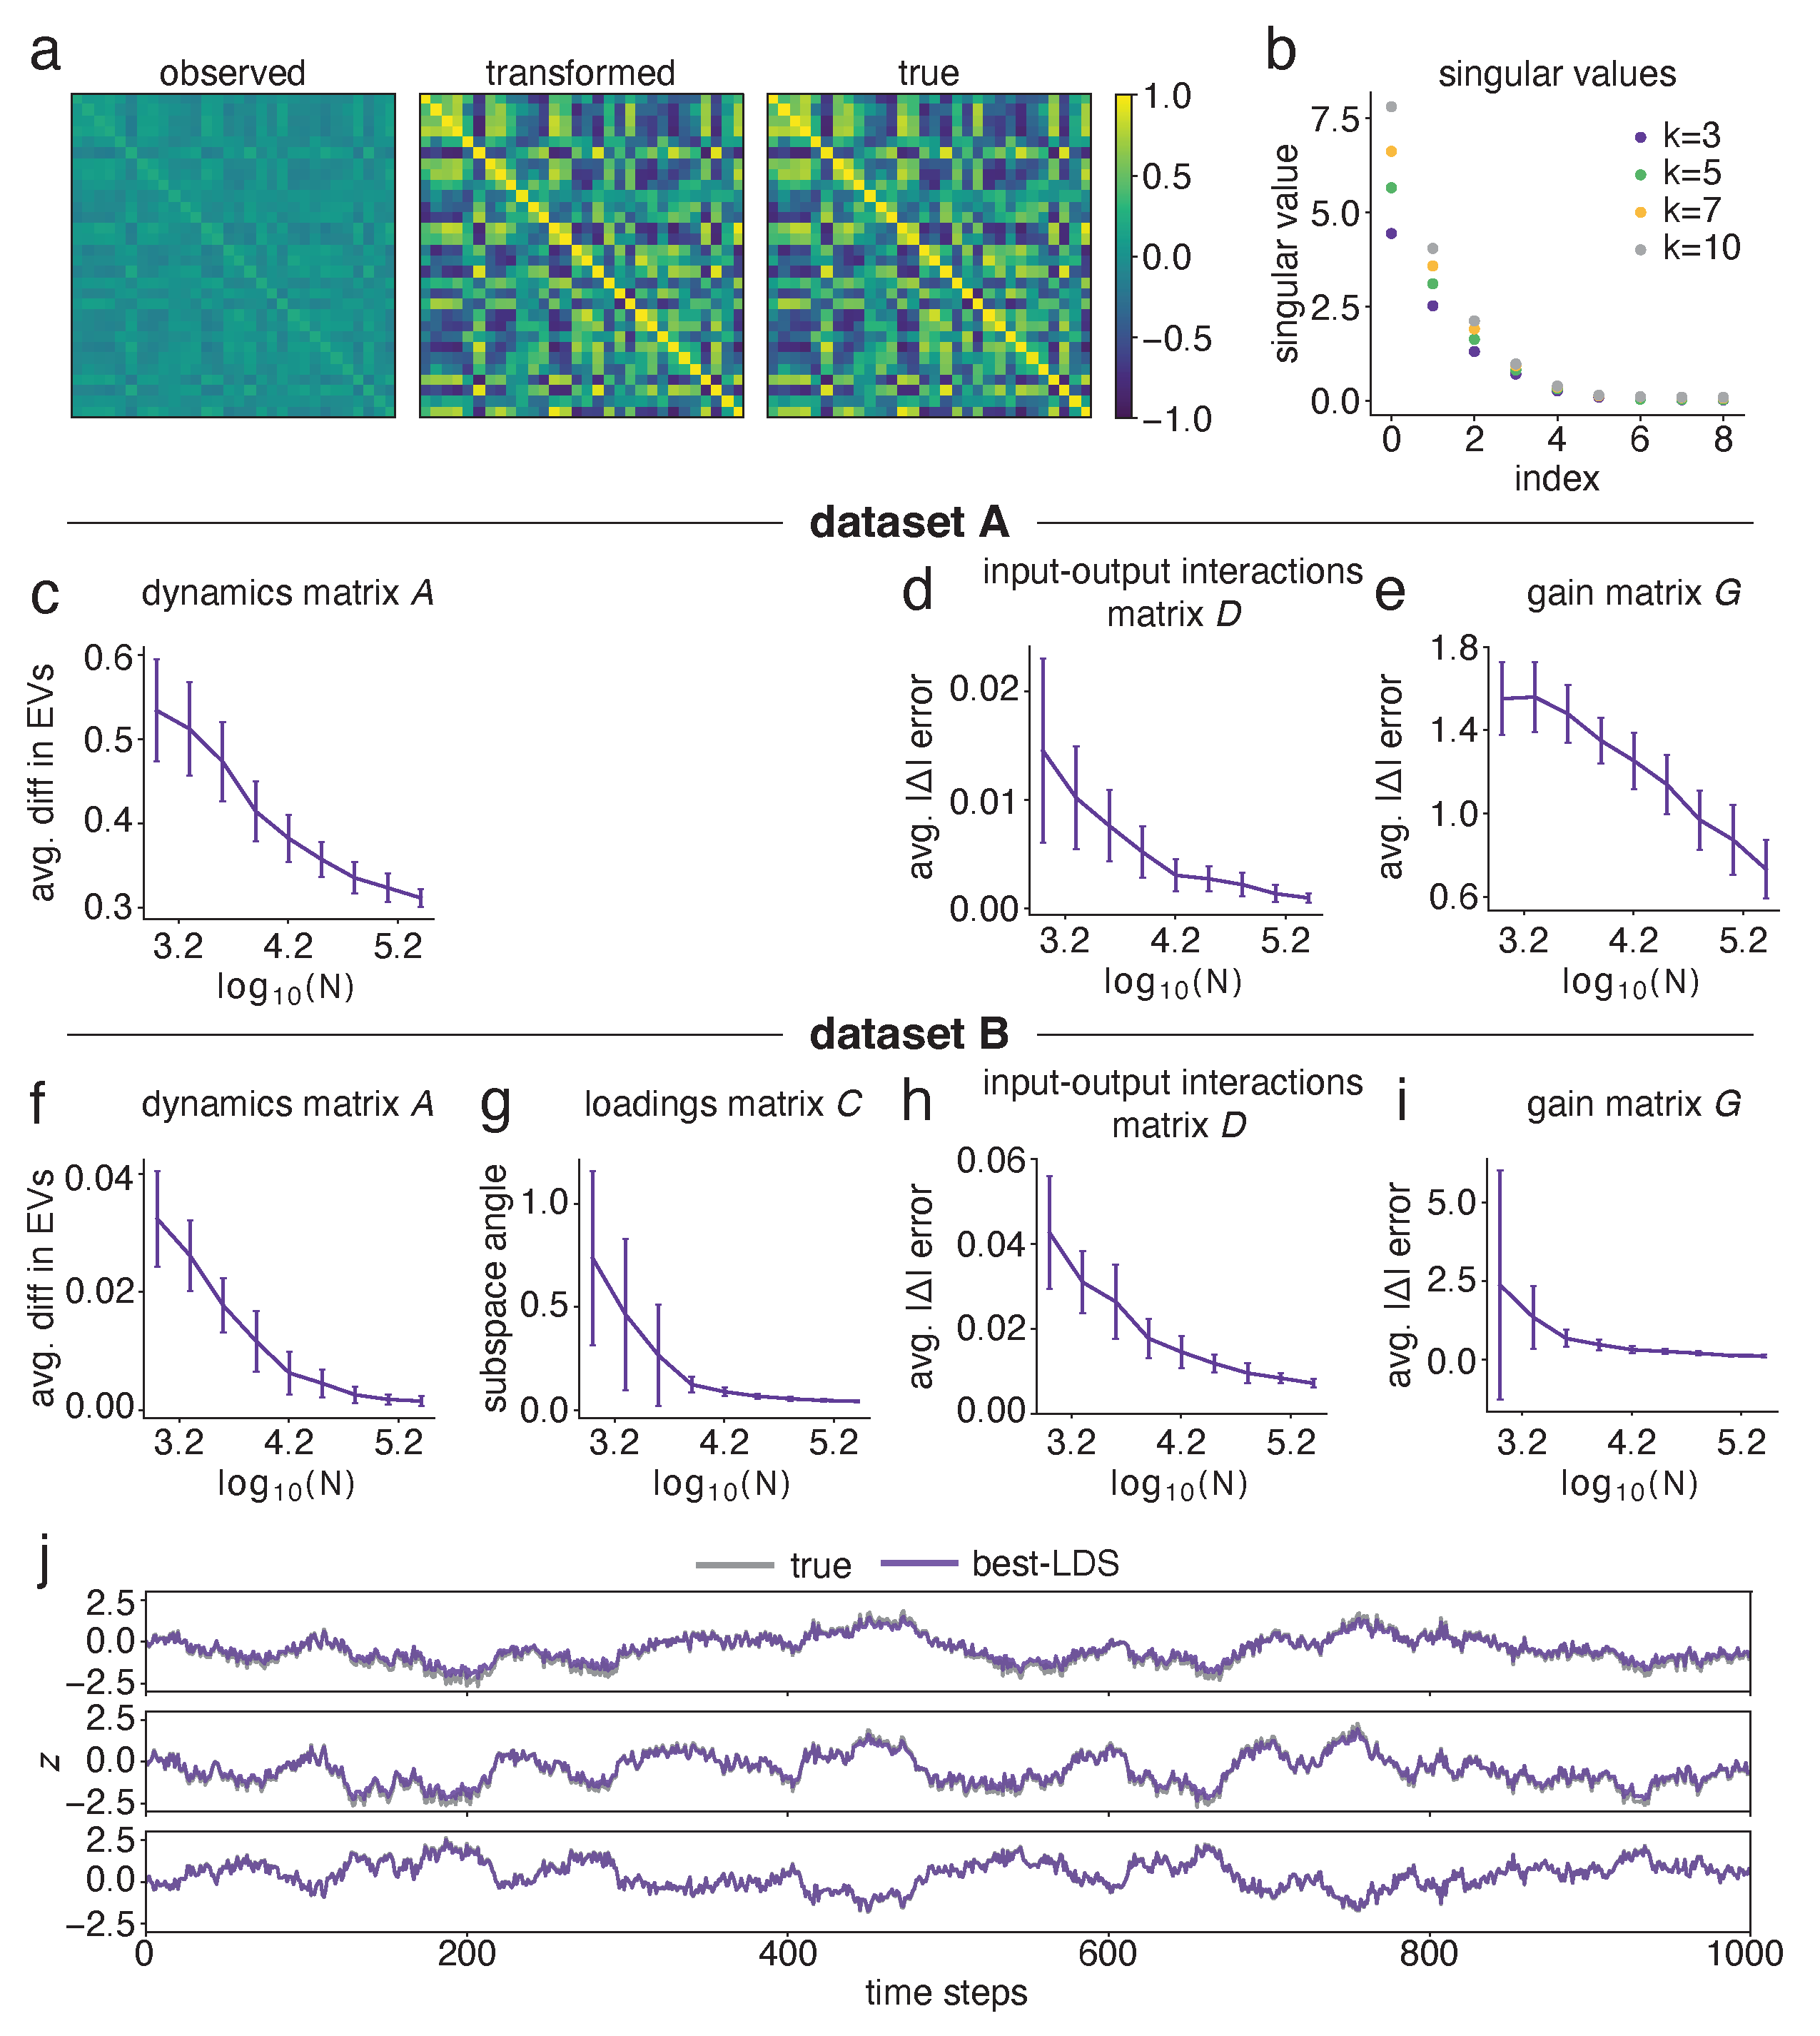
\includegraphics[width=0.90\textwidth]{ch4-bestlds/bestlds-figures/fig2.pdf}
\caption[Spectral estimator recovers simulation parameters in a variety of settings]{\textbf{Spectral estimator recovers simulation parameters in a variety of settings.} \textbf{(a)} Covariance matrix Cov$[y_{t+1}, y_{t}]$ showing the sample covariance of the binary observations $y$ (left), the covariance of $z$ obtained by converting the moments of $y$ (middle), and the ground truth covariance of $z$ (right) for a simulated dataset ($q = 30$, $p = 15$, $k =20$, $m=3$). Note that the transformed covariance closely matches the ground truth. \textbf{(b)} The singular value spectrum of the Hankel matrix computed at various settings of the Hankel size $k$. For all settings, only the top $p=5$ singular values are greater than zero. \textbf{(c-e)} Recovery error for bestLDS inferred parameters vs. training data size for a low-dimensional dataset with $ k=3$. For (c) we use the average absolute difference in the eigenvalues as the recovery error, and for (d) and (e) we use the average absolute elementwise difference. \textbf{(f-i)} Recovery error for bestLDS inferred parameters vs. training data size for a high-dimensional dataset with $k=10$. For (g) the recovery error is the angle of the }
\vspace{-0.5cm}
\label{fig:bestlds:2}
\end{figure*}
\begin{figure}[t!]
  \contcaption{subspaces spanned by $C$ and $\hat{C}$. \textbf{(j)} Latent state trajectories simulated from true and inferred parameters for one of the simulations in dataset B. Both datasets exhibited strong temporal correlations and small interaction terms between the latents/outputs and the inputs. See Appendix Table \ref{table:ap2:1} for more details.}% Continued caption
\end{figure}

Next, we demonstrate the relative insensitivity of our algorithm's performance to the Hankel size $k$ by examining the singular value spectrum of the Hankel matrix, which one can use to determine the proper choice of the latent dimension $p$ for independent analysis or prior to using a fitting method like EM (see section~\ref{sec:bestlds:results:4.3}). For simulated data of $N=256,000$ in which $p=5$, we repeatedly fit bestLDS while varying the Hankel size ($k=[3,5,7,10]$). The results show that the general structure of of the singular value spectrum is independent of $k$ (Figure~\ref{fig:bestlds:2}b). Indeed for all four simulations only the first five singular values are non-zero, consistent with the true structure of the data.  

To illustrate the effectiveness of bestLDS, we next show that the estimator returns consistent, accurate estimates of the generative parameters on two simulated datasets, one low-dimensional and the other high-dimensional. In both datasets, ground-truth data is drawn by simulation from a probit-Bernoulli LDS with $\mu_0=0$ and $Q_0$ taken to be the stationary marginal covariance of the latents. $A, B, $ and $D$ are sampled independently from a standard normal distribution and then have their eigenvalues thresholded (spectral radius $<1$ is needed for $A$ to ensure stability). We take $C$ to be a random orthonormal matrix such that, given $A$, the stationary marginal covariance of $z$ has unit diagonal (results of simulations where we do not make this assumption on the marginal covariance are available in Supplementary Figure~\ref{fig:ap2:1}). 

Note that LDS models are not uniquely identifiable and SSID algorithms in general recover parameters only up to a similarity transformation. Concretely, let $x' = Tx$, for $T$ an invertible matrix. Then we may recover $A' = T^{-1}AT, B' = T^{-1}B$ and $C' = CT^{-1}$. $D$ is recovered canonically and thus we can look at the mean elementwise error to establish the accuracy of our estimator for this matrix. For the other parameters, however, we must establish alternative error metrics. For $A$, we measure the error of its estimate $\hat{A}$ by examining the average absolute difference in their eigenvalues. For $C$, we look at the angle between the subspaces spanned by the true $C$ and the estimate $\hat{C}$. For $B$, there is not a simple error metric.  However, we can examine the gain matrix $G = C(I-A)^{-1}B + D$, which is preserved canonically under the similarity transformation, taking the mean absolute difference across the inferred and true gain matrices as an overall indicator of accuracy in the recovery process. For both datasets, we computed these error metrics and took their average across $30$ simulations for $N \in [1000, 256000]$. The time taken to run bestLDS on these datasets is available in Supplementary Figure~\ref{fig:ap2:2}.

\begin{table}[t]
\centering
\setlength{\tabcolsep}{4.2pt}
 \caption[Comparison of the mean log-evidence for inferred and true parameters across three different datasets]{\textbf{Comparison of the mean log-evidence for inferred and true parameters across three different datasets.} Data was simulated using a trial structure such that every trial corresponded to a unique test set, with five total trials. The number of data points listed in the table corresponds to the full size of the dataset (so each trial/test set was $N=10k$ and $N=51.2k$, respectively). See Appendix Table \ref{table:ap2:1} for details on simulation parameters. }
 \vspace{0.2cm}
\begin{tabular}{ |p{2.1cm}||p{1.4cm}|p{1.4cm}|p{1.4cm}|p{1.4cm}|p{1.4cm}|p{1.4cm}|}
 \hline
 \multicolumn{7}{|c|}{\textbf{Model Comparisons} } \\
 \hline
 \multirow{2}{0em}{\textbf{Method}} & \multicolumn{2}{|c|}{\textbf{Dataset A*}} & \multicolumn{2}{|c|}{\textbf{Dataset B}} & \multicolumn{2}{|c|}{\textbf{Dataset C}} \\ 
 \cline{2-7}
& \textbf{50k} & \textbf{256k} & \textbf{50k} & \textbf{256k} & \textbf{50k} & \textbf{256k} \\
 \hline
 \textbf{true}  &   -1521  & -9906 &  -38254   &   -190063 & -41161 & -211821 \\
 \textbf{bestLDS}  & -238  & -4456  & -32139 & -159129 &  -40269 & -207713 \\
 \textbf{pLDS}   &    N/A &    N/A  & -41732 & -197463 &  -42799 &  -226886 \\
 \textbf{gaussLDS}   & -255 &  -5636 & -39291 & -205960 &  -43556 &   -228090 \\
 \hline
\end{tabular}
\vspace{-0.35cm}
\label{table:bestlds:1}
\end{table}

The accuracy of the system matrices recovered via bestLDS are displayed in Figure ~\ref{fig:bestlds:2}c-i. In the low-dimensional dataset (dataset A), the errors for each relevant error metric decrease with increasing data size (note subspace angle is not possible to compute for $C$ when $q<p$). While the errors for $A$ and $G$ are non-zero even at $N=256000$, systems in which $q < p$ (i.e. high-dimensional latent structure governs low-dimensional outputs), are a particular challenge for LDS models. Therefore it is notable that we nonetheless see decreasing errors---and for certain metrics quite small errors---in this regime. As a contrasting example, we simulated a high-dimensional dataset with higher-dimensional latent dynamics (dataset B). Our estimator performs extremely well in this regime. For the system matrices $A$, $C$, and $D$ as well as the gain matrix $G$ (Figure~\ref{fig:bestlds:2}f-i), the error metrics decay to zero, indicating that our estimator is consistent. Furthermore, the errors are quite low across the whole range of dataset-sizes taken---for example, the mean error in $A$ at $N=1000$ is less than $0.05$. For completeness, we compared the accuracy of our estimator against running N4SID directly on $z$ (i.e., pretending we have access to the Gaussian subset of the LDS and therefore forgoing the need to perform moment conversion) and found that bestLDS did not perform significantly worse on most variables (Supplementary Figure~\ref{fig:ap2:3}). Thus our estimator is quite effective, even in a sparse-data regime. To further validate our parameter recovery for dataset B, we simulated noiselessly using both the true and inferred parameters and found that the latent state traces overlapped almost exactly (Figure~\ref{fig:bestlds:2}g). 

Lastly, we performed model comparisons on three datasets of different sizes to illustrate the accuracy of our recovery process in different settings (Table~\ref{table:bestlds:1}). Dataset B has the same simulation parameters as in Figure~\ref{fig:bestlds:2}. Dataset C has lower autocorrelations, larger instantaneous correlations, and similarly small input-latent/output interactions. Dataset A* is the average over 10 datasets with the same generative parameters as dataset A;  we did this to make our model comparison results more robust given the peculiarities of the $q<p$ regime. Using the Laplace approximation\footnote{While the simulated data is generated from a probit-Bernoulli model, the inference code used to compute the log-evidences assumes a logit model. To address this inconsistency, we adjusted the inference code to account for a scale factor on the observation parameters C and D to align the probit and logit models.}, we computed the log-evidence given the true parameters, the bestLDS inferred parameters, the inferred parameters using the Poisson LDS (pLDS) estimator as detailed in \cite{buesing_spectral_2012}, and the inferred parameters using a linear-Gaussian (gaussLDS) estimator\footnote{computed by treating the binary data as real-valued and simply fitting a Gaussian LDS to the data using N4SID (i.e., skipping the moment conversion step)}. In the cases we have examined, bestLDS achieves the highest log-evidence amongst the benchmarks tested, indicating that the bestLDS parameters can suffice on their own in capturing the characteristics of the system even without subsequent optimization. This also demonstrates the need for estimators that account for the specific distribution of the underlying data, as it is not sufficient to simply substitute a different estimator and achieve accurate results. 